\documentclass[11pt]{beamer}

%%%%%%%% tema e cor %%%%%%%%
\mode<presentation> {
\usetheme{Madrid}
%\usecolortheme{albatross}
}

\usepackage[utf8]{inputenc}
\usepackage{graphicx} 
\usepackage{booktabs} 
\usepackage[options ]{algorithm2e}

\date{\today}

\AtBeginSection[]
{
\begin{frame}
\frametitle{Curriculum Plan}
\tableofcontents[currentsection]
\end{frame}
}

%%%%%%%% titulo e subtitulo %%%%%%%%
\title[AI4ALL Computer Vision]{Image Representation and Neural Networks} 

%%%%%%%% nome dos autores %%%%%%%%
\author[Andrew Kondrich]{Andrew Kondrich} 

\begin{document}
\begin{frame}
\titlepage 

\end{frame}

\begin{frame}
\frametitle{Class schedule} 
\tableofcontents 
\end{frame}

%%%%%%%% slides %%%%%%%%
\section{Linear Models for Regression and Classification}
\begin{frame}{Linear Models for Regression}
    \begin{figure}
    \centering
    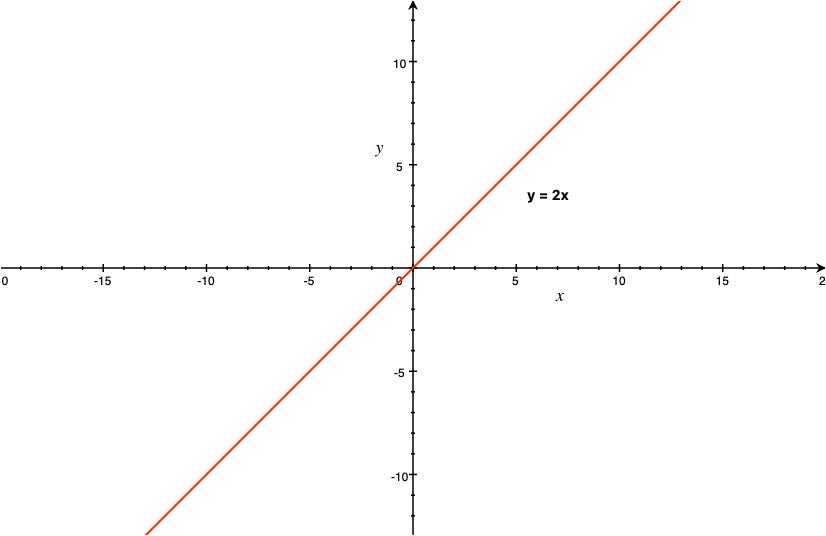
\includegraphics[width=.7\textwidth]{img/line.jpg}
    \caption{$y$ is given as a function of $x$ in the form $y=mx+b$}
    \end{figure}
\end{frame}

\begin{frame}{Linear Models for Regression}
\begin{itemize}
    \item Data is a collection of paired points such as
    $$(0, 0), (1, 1), (2.5, 2), (5, 6), ...$$
    \item We assume data can be fit by a linear hypothesis function
    $$y = w_1x + b$$
    \item \textbf{Our job:} Given just this data, how to choose $w_1$ and $b$?
\end{itemize}
\end{frame}

\begin{frame}{Linear Models for Regression}
\begin{figure}
    \centering
    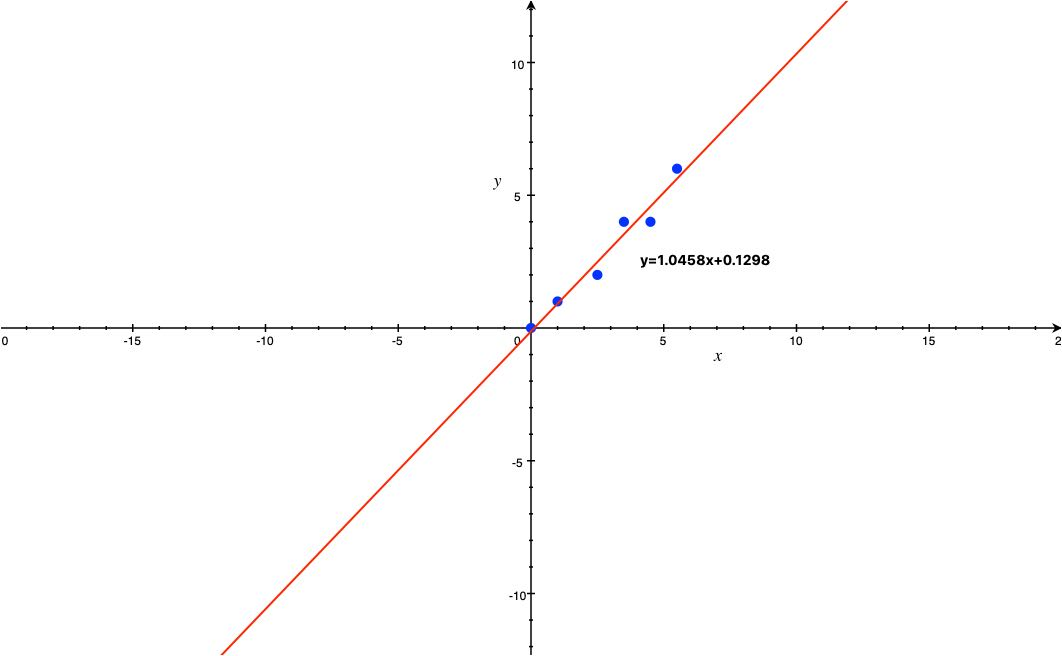
\includegraphics[width=.7\textwidth]{img/regressed_points.jpg}
    \caption{Line interpolated for 2D blue point dataset}
\end{figure}
\end{frame}

\begin{frame}{Linear Models for Regression}
\begin{itemize}
    \item First, we generalize the problem statement a little bit...
    \item You can have more than just one feature $x$.
    \item Instead of just using $ft^2$ to predict price of house, you also include which city your house is in because apartment in San Francisco is small but expensive!
    \item Data of any number of $x$ can be fit by a linear hypothesis function 
    $$y = w_0 + w_1x_1 + ... + w_Dx_D$$
\end{itemize}
\end{frame}

\begin{frame}{Linear Models for Regression}
\begin{figure}
    \centering
    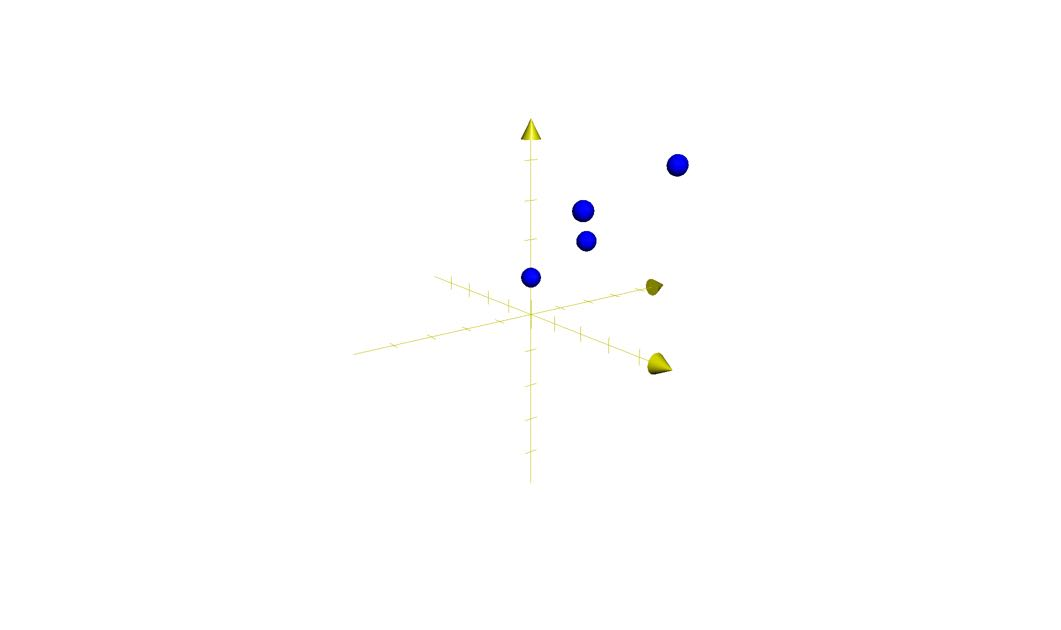
\includegraphics[width=0.9\textwidth]{img/3d_regressed_points.jpg}
    \caption{3D blue point dataset $(x_1, x_2, y)$}
\end{figure}
\end{frame}

\begin{frame}{Linear Models for Regression}
\begin{figure}
    \centering
    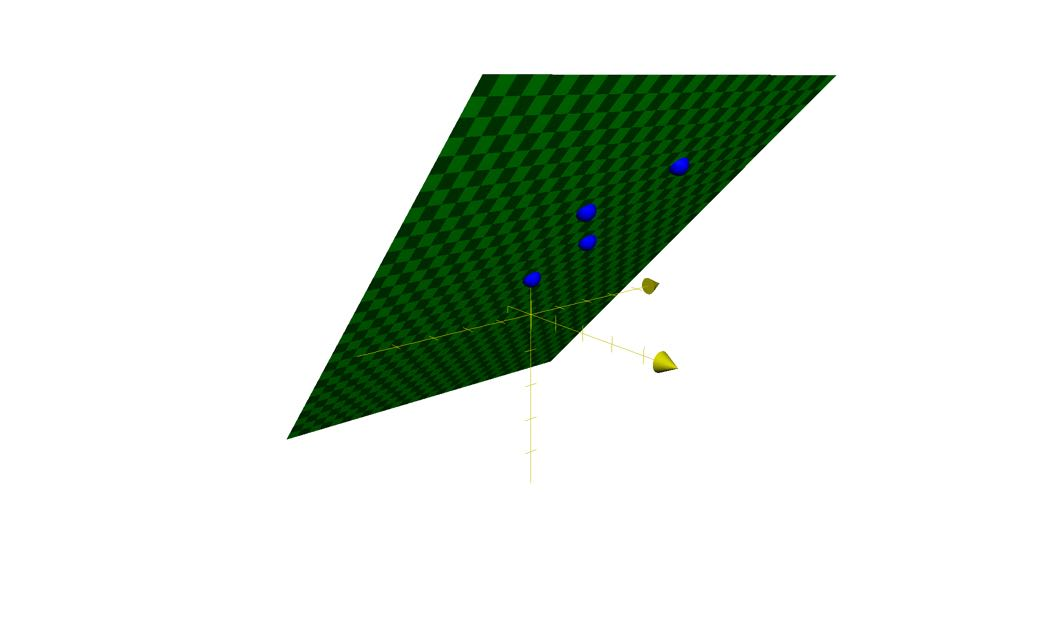
\includegraphics[width=0.9\textwidth]{img/3d_regressed_line.jpg}
    \caption{Regressed \textit{plane}: $y= x_1 - x_2 +1$}
\end{figure}
\end{frame}

\begin{frame}{Linear Models for Classification}
\begin{itemize}
    \item In the regression case, we take input $(x_1, x_2, ..., x_D)$ and return the point $y$ that fits our linear hypothesis function $$y = w_0 + w_1x_1 + ... + w_Dx_D$$ where
    $$y, x_1, x_2, ..., x_D \in \mathbb{R}$$
    \item The goal in classification is to take input $(x_1, x_2, ..., x_D)$ and assign it to one of $K$ groups.
    \item Example of K = 2?
\end{itemize}
\end{frame}

\begin{frame}{Linear Models for Classification}
\begin{itemize}
    \item In the regression case, we take input $(x_1, x_2, ..., x_D)$ and return the point $y$ that fits our linear hypothesis function $$y = w_0 + w_1x_1 + ... + w_Dx_D$$ where
    $$y, x_1, x_2, ..., x_D \in \mathbb{R}$$
    \item The goal in classification is to take input $(x_1, x_2, ..., x_D)$ and assign it to one of $K$ groups.
    \item Example of $K = 2$? 
    
    pass/fail, win/lose, healthy/sick, poor/not poor, hotdog/not hotdog,
    \item We will continue to focus on $K = 2$ case, known as \textbf{binary classification}.
\end{itemize}
\end{frame}

\begin{frame}{Linear Models for Classification}
\begin{itemize}
    \item Regression returns the "real" numeric value we want, e.g. house price in dollars.
    \item Less intuitive: How to capture "group assignment" numerically? 
\end{itemize}
\end{frame}

\begin{frame}{Linear Models for Classification}
\begin{itemize}
    \item Regression returns the "real" numeric value we want, e.g. house price in dollars.
    \item Less intuitive: How to capture "group assignment" numerically? 
    \item Classification models return the \textbf{probability} that input belongs to a group.
\end{itemize}
\end{frame}

\begin{frame}{Linear Models for Classification}
\begin{itemize}
    \item Regression returns the "real" numeric value we want, e.g. house price in dollars.
    \item Less intuitive: How to capture "group assignment" numerically? 
    \item Classification models return the \textbf{probability} that input belongs to a group.
    \item For binary classification: We need to find some function $f$ defined as $$p = f(x_1, x_2, ..., x_D)$$ that takes $(x_1, ..., x_D)$, does some math, and returns a probability $p$ of belonging to Group 1.
    \item Probability of being in Group 2 is given by $1-p$.
\end{itemize}
\end{frame}

\begin{frame}{Linear Models for Classification}
\begin{itemize}
    \item We use a modified version of our linear regression function:
    $$y = \sigma(w_0 + w_1x_1 + ... + w_Dx_D)$$
    \item Where $\sigma$ is the \textbf{sigmoid} function, a type of logistic funciton given by
    $$\frac{1}{1 + e^{-x}}$$
    \item In statistics, this model is known as \textbf{logistic regression}, although it should be emphasized that this is a model for classification rather than regression.
\end{itemize}
\end{frame}

\begin{frame}{Linear Models for Classification}
\begin{figure}
    \centering
    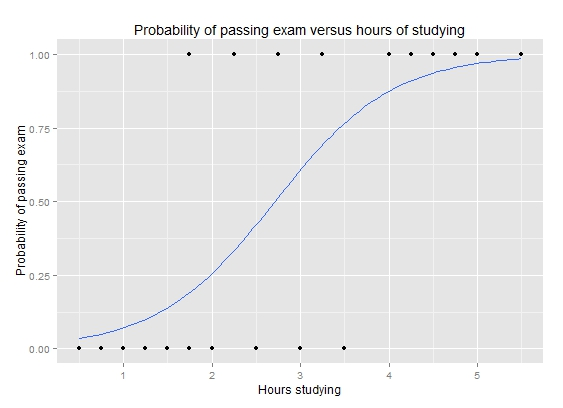
\includegraphics[width=0.7\textwidth]{img/Exam_pass_logistic_curve.jpeg}
    \caption{\label{fig:researchscope}By Michaelg2015 - Own work, CC BY-SA 4.0, https://commons.wikimedia.org/w/index.php?curid=42442194}
\end{figure}
\end{frame}


\section{Optimization}
\begin{frame}{Optimization}
\begin{itemize}
    \item We know how to represent our logistic and linear regression functions:
    $$y =(w_0 + w_1x_1 + ... + w_Dx_D)$$
    $$y = \sigma(w_0 + w_1x_1 + ... + w_Dx_D)$$
    \item We need some algorithm for finding what the best choices of $(w_0, ..., w_D)$ are.
    \item \textbf{Gradient Descent} is a process by which we iteratively improve our choices for $(w_0, ..., w_D)$ by computing the \textbf{gradient} of the \textbf{loss} of our predictions.
\end{itemize}
\end{frame}

\begin{frame}{Optimization}
\begin{itemize}
    \item \textbf{Gradients} equal the slope of the line that is \textit{tangent} to your function.
    \item Imagine that one of these lines exists for each point along your function.
    \begin{figure}
    \centering
    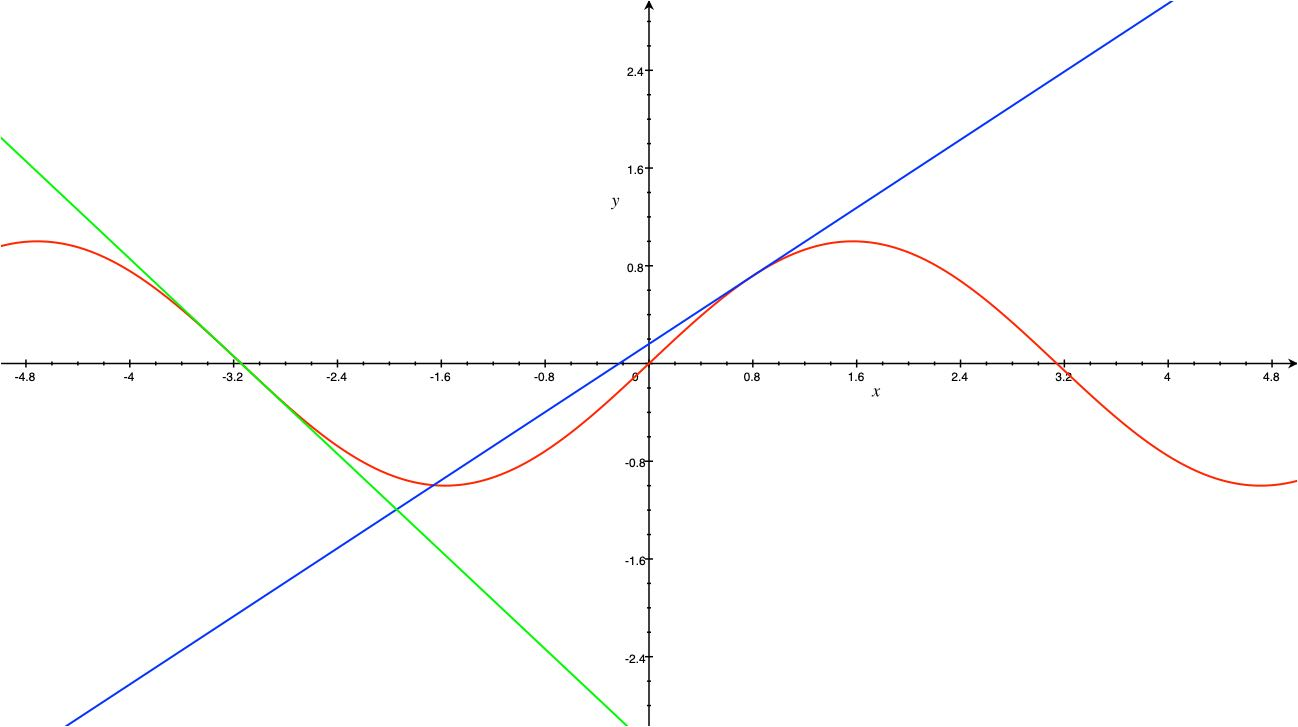
\includegraphics[width=0.6\textwidth]{img/TwoTangentLine.jpg}
    \caption{Lines tangent to $y = sin(x)$ at $x = 0.8$ and $x=-3.2$}
    \end{figure}
    \item They indicate the direction in which the function is increasing.
    
\end{itemize}
\end{frame}

\begin{frame}{Optimization}
    \begin{center}
    \item Physical Metaphor: The function is a hill. A \textbf{positive} gradient indicates a ball would roll \textbf{left}, a negative gradient indicates a \textbf{ball} would roll \textbf{right}.
    \end{center}
\end{frame}

\begin{frame}{Optimization}
\begin{itemize}
    \item A common loss function is the \textbf{Mean Squared Error} $\mathcal{L}(y, \hat{y}) = (y - \hat{y})^2$. Why do you think that is?
\end{itemize}
\end{frame}

\begin{frame}{Optimization}
\begin{itemize}
    \item A common loss function is the \textbf{Mean Squared Error} $\mathcal{L}(y, \hat{y}) = (y - \hat{y})^2$. Why do you think that is?
    \begin{figure}
    \centering
    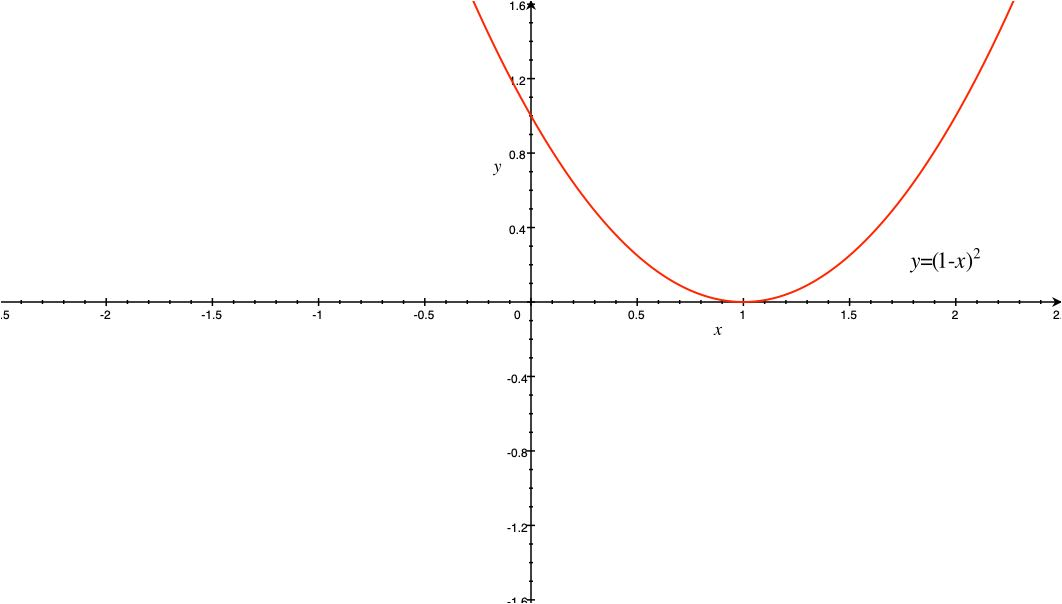
\includegraphics[width=0.6\textwidth]{img/MSELoss.jpg}
    \caption{Graph of $y=(1-x)^2$}
    \end{figure}
\end{itemize}
\end{frame}

\begin{frame}{Optimization}
    \begin{figure}
    \centering
    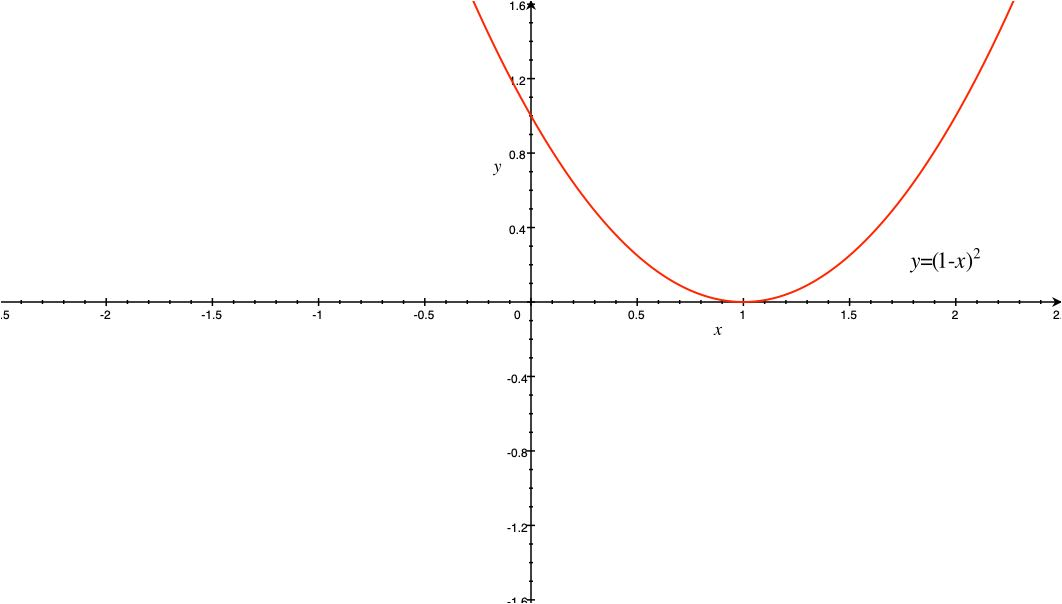
\includegraphics[width=0.8\textwidth]{img/MSELoss.jpg}
    \caption{Graph of $y=(1-x)^2$} or $\mathcal{L}(y=1, \hat{y}) = (1-\hat{y})^2$
    \end{figure}
\end{frame}

\begin{frame}{Optimization}
\begin{itemize}
    \item \textbf{Mean Squared Error} (MSE) defined by $\mathcal{L}(y, \hat{y}) = (y - \hat{y})^2$. 
    \item What is $\hat{y}$? Its the output of linear or logistic regression!
    $$\hat{y} =(w_0 + w_1x_1 + ... + w_Dx_D)$$
    $$\hat{y} = \sigma(w_0 + w_1x_1 + ... + w_Dx_D)$$
    \item $y$ is the corresponding label to datapoint $(x_1, x_2, ..., x_D)$!
\end{itemize}
\end{frame}

\begin{frame}{Optimization}
    \begin{itemize}
        \item Collect a dataset of $(y, x_1, x_2, ..., x_D)$ sequences.
        \item Choose some initial weights randomly, $(w_0, w_1, ..., w_D)$
    \end{itemize}
    \begin{algorithm}[H]
    \SetAlgoLined
     \While{loss is not absolute minimum}{
      find $\hat{y} = \sigma(w_0 + w_1x_1 + ... + w_Dx_D)$ for each $(y, x_1, x_2, ..., x_D)$\;
      compute MSE $\mathcal{L}(y, \hat{y}) = (y - \hat{y})^2$\;
      recompute weights using \textbf{gradient} of your loss (shows direction to nudge your weights)\;
     }
     \caption{Gradient Descent Algorithm for Binary Classification}
    \end{algorithm}
    % \textbf{Gradient Descent algorithm procedure}
    % \item 
    % \item Solve either logistic or linear regression
    % $$\hat{y} =(w_0 + w_1x_1 + ... + w_Dx_D)$$
    % $$\hat{y} = \sigma(w_0 + w_1x_1 + ... + w_Dx_D)$$
    % \item Compute MSE $\mathcal{L}(y, \hat{y}) = (y - \hat{y})^2$
    % \item 
    
% \end{itemize}
    
\end{frame}

\section{Vectors}
\begin{frame}{Vectors}
\begin{itemize}
    \item Recap: Vectors are a sequence of numbers
    $$[1.0, 2.0]; [6.0, 5.3, 2.1, -6.7]$$
    \item Vector Spaces
    $$\mathbb{R}^2 = \{(x, y) : x, y \in \mathbb{R}\}$$
    $$\mathbb{R}^4 = \{(a, b, c, d) : a, b, c, d \in \mathbb{R}\}$$
    \begin{figure}
    \centering
    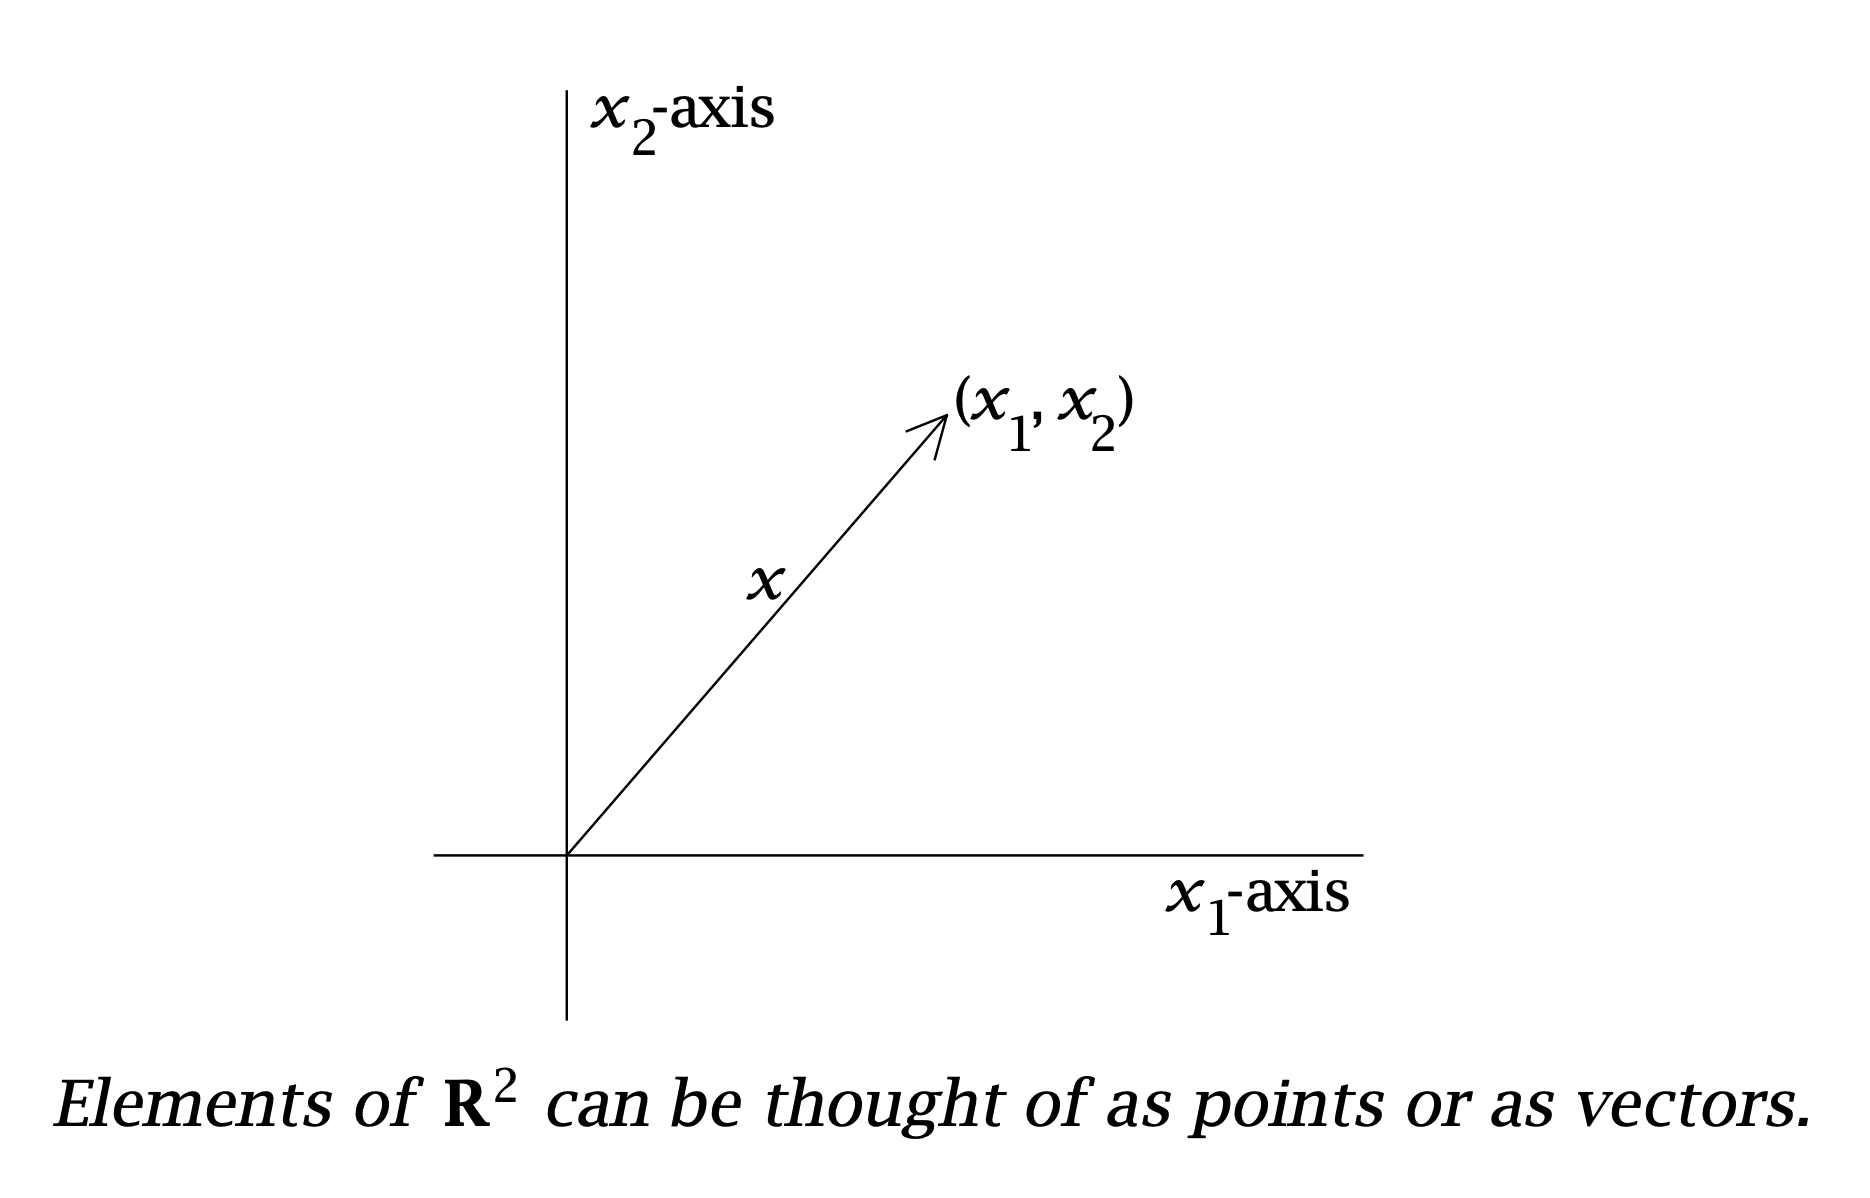
\includegraphics[width=.5\textwidth]{img/vectors.png}
    \end{figure}
\end{itemize}
\end{frame}

\begin{frame}{Linear Models for Regression}
\begin{figure}
    \centering
    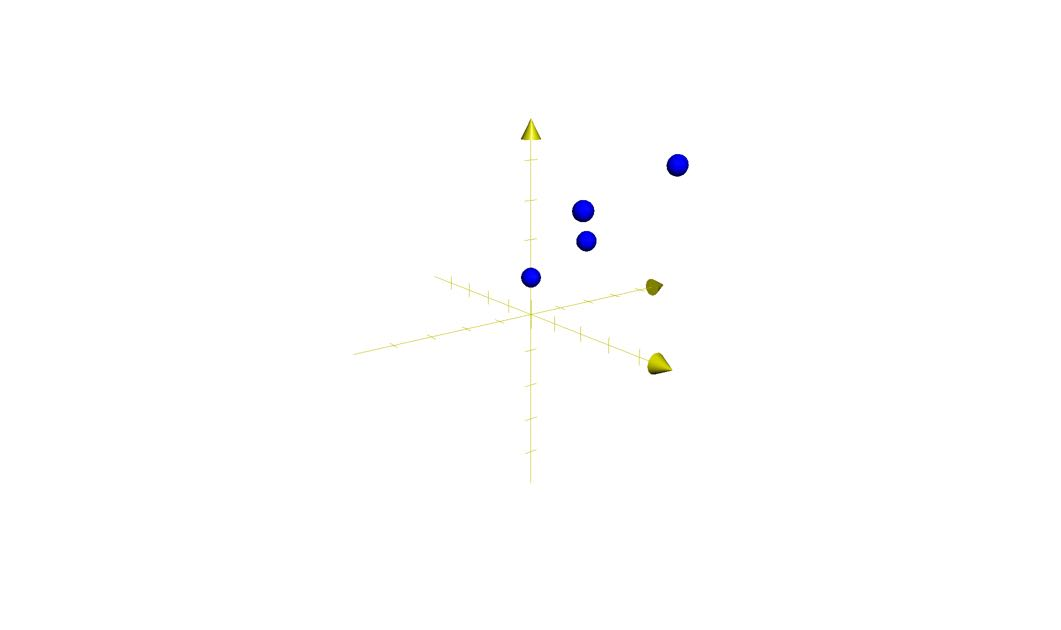
\includegraphics[width=0.9\textwidth]{img/3d_regressed_points.jpg}
    \caption{3D blue point dataset $(x_1, x_2, y) \in \mathbb{R}^3$}
\end{figure}
\end{frame}

\begin{frame}{Vectors}
\begin{itemize}
    \item In logistic regression: $\hat{y} = \sigma(w_0 + w_1x_1 + ... + w_Dx_D)$
    $$\textbf{w} = (w_0, ..., w_D) \in \mathbb{R}^D, \textbf{x} = (x_0, ..., x_D) \in \mathbb{R}^D$$
    $$\hat{y} = \sigma(\textbf{w} \cdot \textbf{x})$$
\end{itemize}
\end{frame}



\section{Matrices}
\begin{frame}{Matrices}
\begin{itemize}
    \item An $m$-by-$n$ matrix is a rectangular array with $m$ rows and $n$ columns that looks like this:
    \begin{figure}
    \centering
    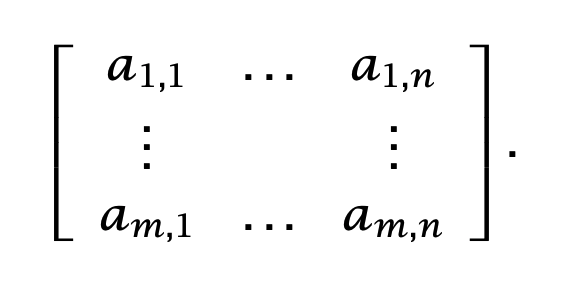
\includegraphics[width=.5\textwidth]{img/matrix.png}
    \end{figure}
    \item Use matrices to represent collections of data (each row is a vector)
    \item Matrices can represent images
\end{itemize}
\end{frame}

\begin{frame}
    \begin{figure}
    \centering
    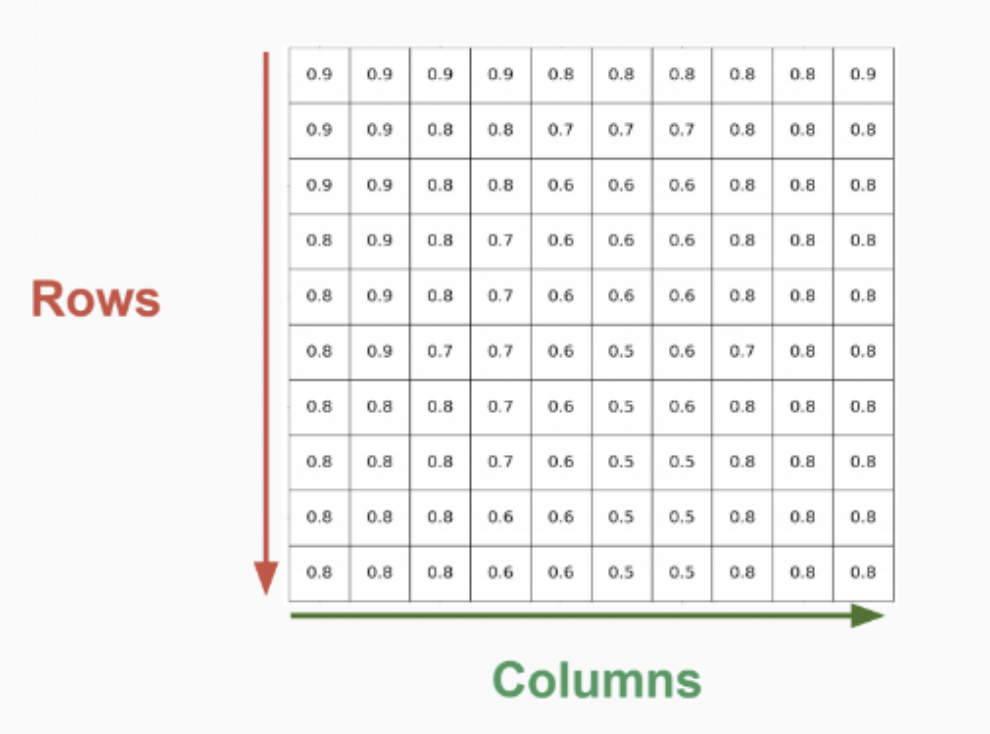
\includegraphics[width=.7\textwidth]{img/num_matrix.png}
    \caption{An example matrix filled with numbers}
    \end{figure}
\end{frame}

\section{Image Representation}
\begin{frame}{Image Representation}
\begin{figure}
    \centering
    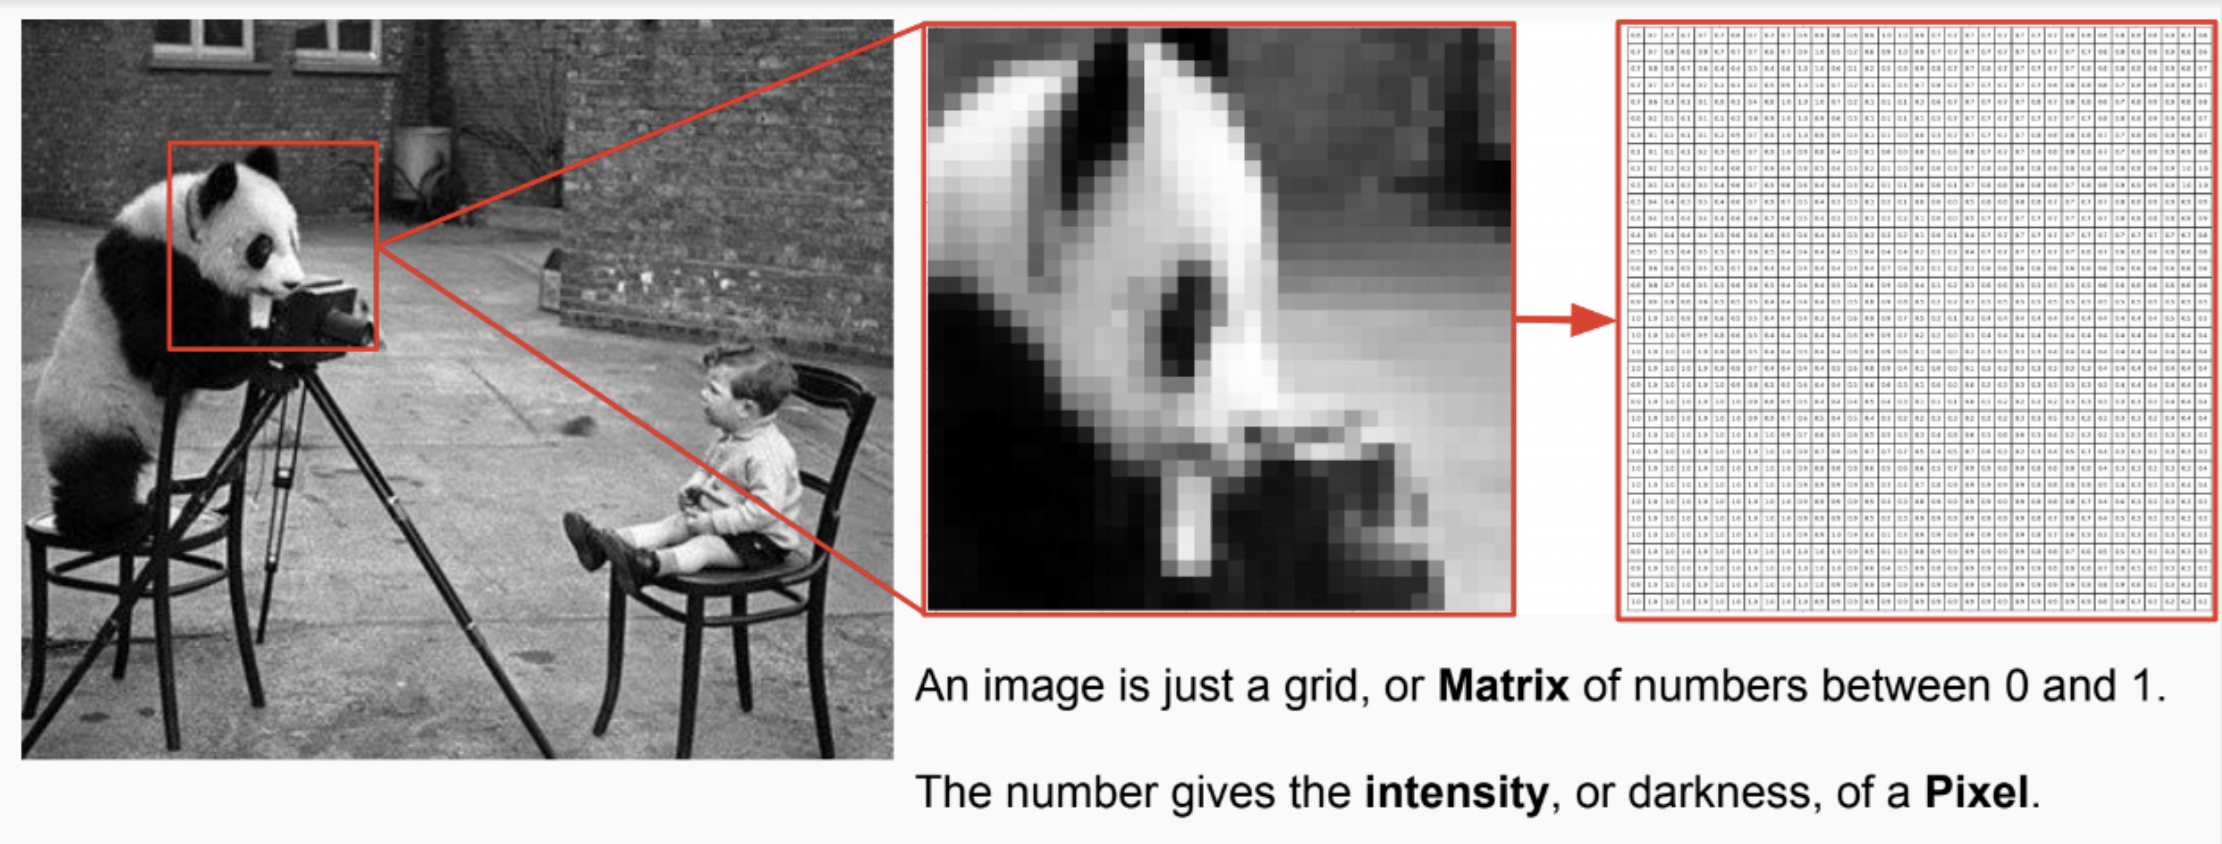
\includegraphics[width=0.9\textwidth]{img/greyscaleimage.png}
    \caption{Black \& White image of panda is a matrix}
\end{figure}
\end{frame}

\begin{frame}{Representing Color}
\begin{figure}
    \centering
    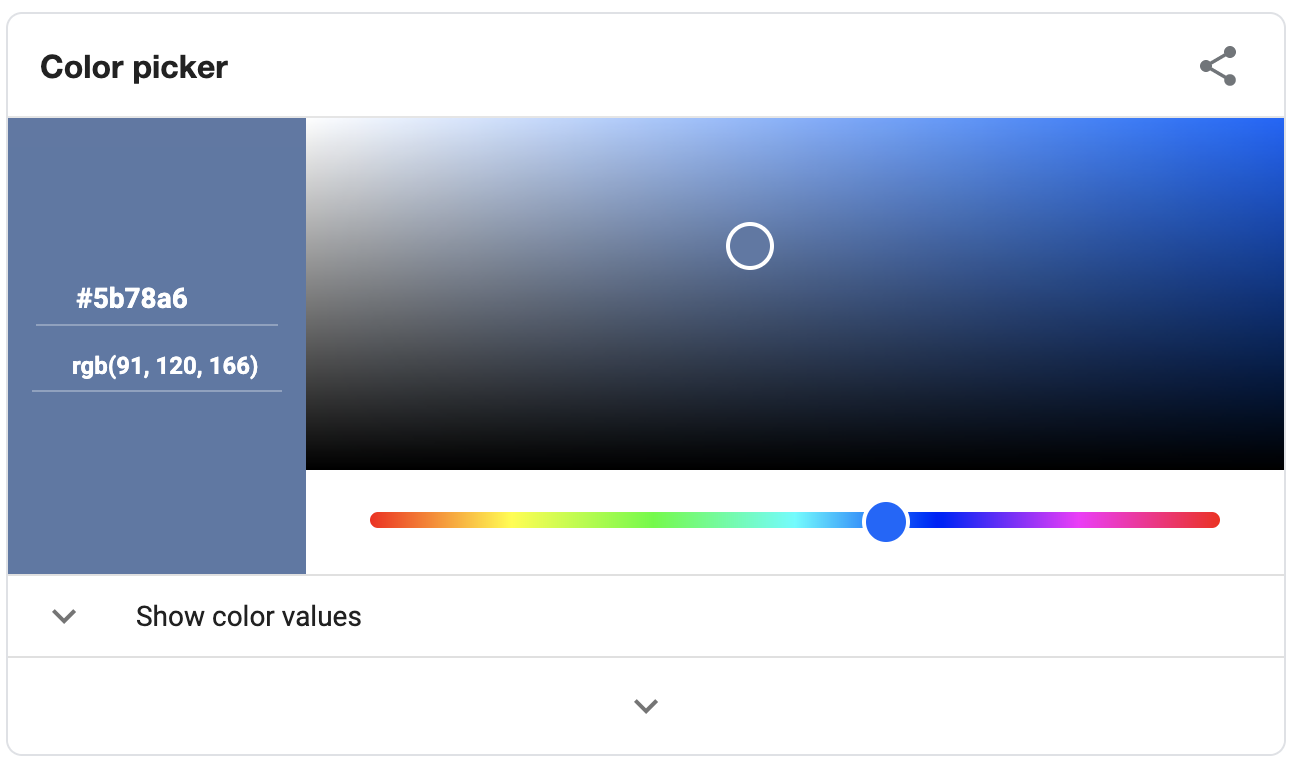
\includegraphics[width=0.9\textwidth]{img/colorpicker.png}
    \caption{Color of single pixel is represented by combination of 3 RGB values}
\end{figure}
\end{frame}

\begin{frame}{Representing Color}
\begin{figure}
    \centering
    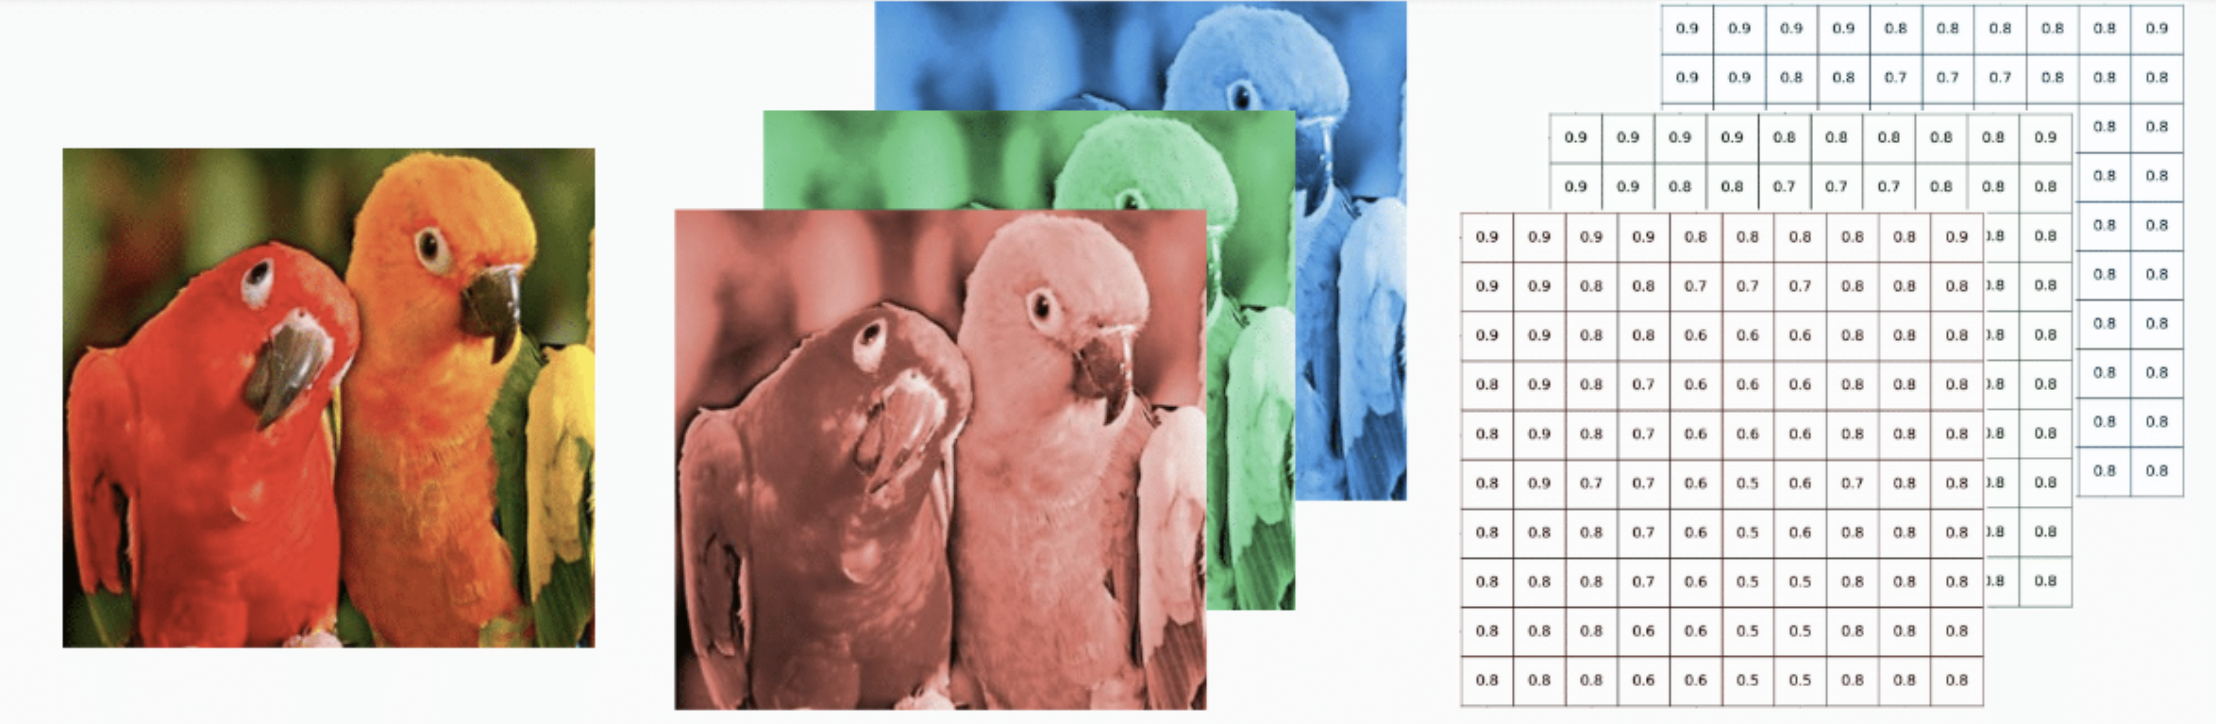
\includegraphics[width=0.9\textwidth]{img/rgbparrot.png}
    \caption{Stacking RGB layers forms final picture}
\end{figure}
\end{frame}

\begin{frame}{Representing Color}
\begin{figure}
    \centering
    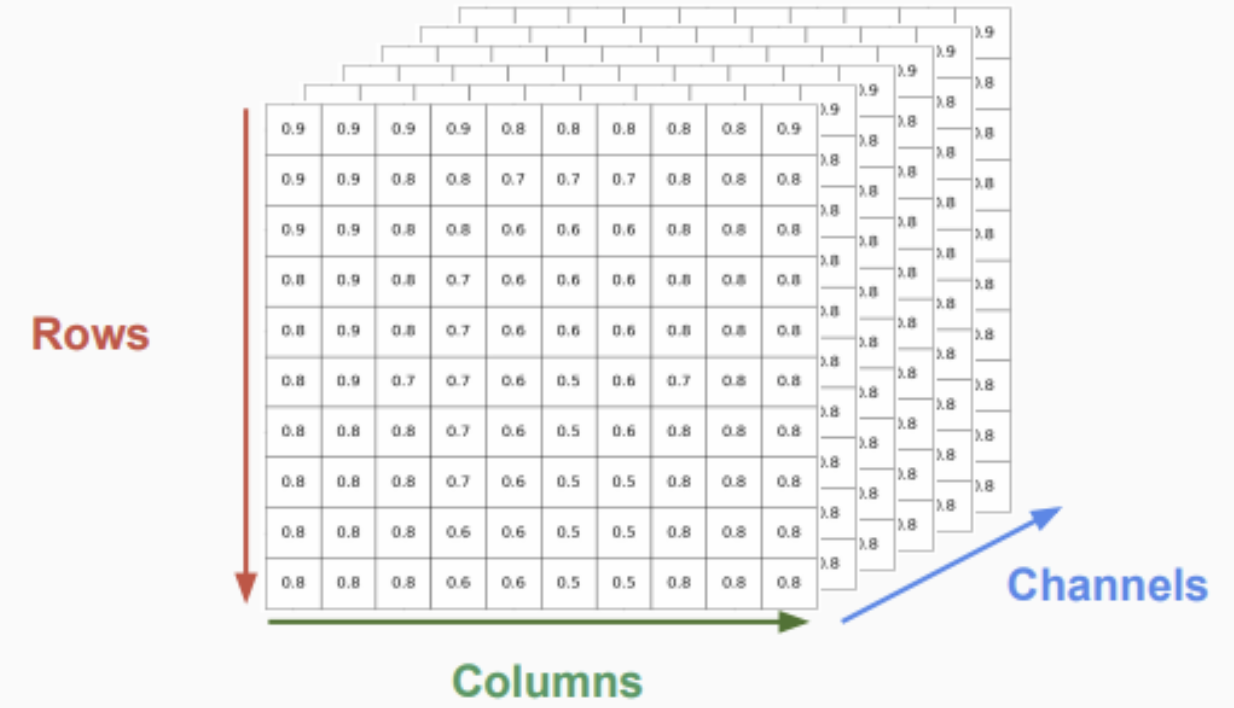
\includegraphics[width=0.7\textwidth]{img/rowcolchannel.png}
    \caption{Numerically, images are 3-dimensional matrices with rows, columns, and 3 \textbf{channels}. We also call these \textbf{volumes}.}
\end{figure}
\end{frame}

\section{Image Classification}
\begin{frame}{Image Classification}
\begin{itemize}
    \item We can represent an image as a vector in a very high dimensional space, $\mathbb{R}^D$
    \begin{figure}
    \centering
    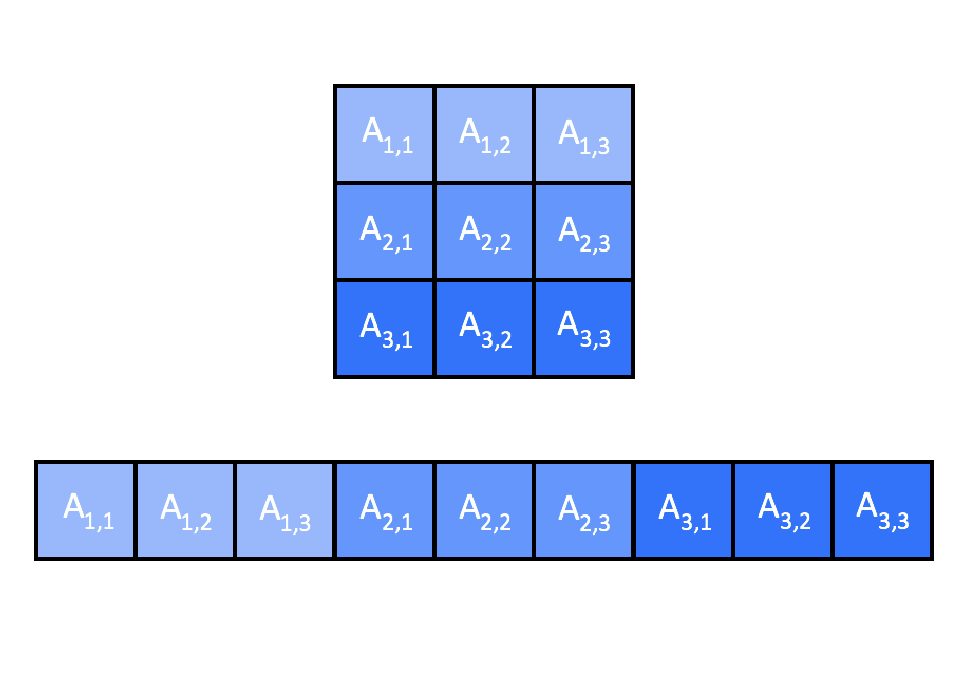
\includegraphics[width=0.6\textwidth]{img/flatten.png}
    
    \caption{Flatten a matrix $A$ into a vector\footnote{quantstart.com}}
    \end{figure}
\end{itemize}

\end{frame}

\begin{frame}{Image Classification}
\begin{itemize}
    \item After flattening image $\textbf{x} \in \mathbb{R}^D$, we want to classify as cat/ not cat using logistic regression
    $$y = \sigma(w_0 + w_1x_1 + ... + w_Dx_D)$$
    where each $x_i \in \textbf{x}$ is a value for one pixel in one RGB channel.
    \begin{figure}
    \centering
    
\includegraphics[width=0.6\textwidth]{img/cat.jpg}
    \end{figure}
    \item What could be a problem with this approach?
\end{itemize}
\end{frame}

\begin{frame}{Image Classification}
\begin{itemize}
    \item Interpretation of linear classifiers as template matching. 
    \item Weights W corresponds to a template for the cat class. 
    \item Whether or not an image is a cat is decided by comparing the template with the image using dot product to find if the score exceeds the $0.5$ decision boundary.
\end{itemize}
\end{frame}

\begin{frame}{Image Classification}
    \begin{figure}
    \centering
    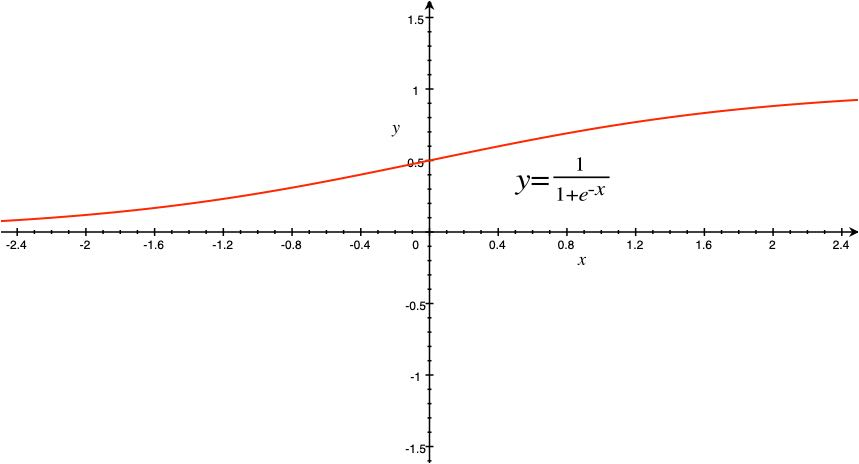
\includegraphics[width=0.8\textwidth]{img/sigmoid.jpg}
    \caption{The sigmoid function $\sigma$ will predict cat for higher value of $\textbf{x} \cdot \textbf{w}$, and not cat for lower.}
    \end{figure}
\end{frame}

\begin{frame}{Image Classification}
\begin{itemize}
    \item Interpretation of linear classifiers as template matching. 
    \item Weights W corresponds to a template for the cat class. 
    \item Whether or not an image is a cat is decided by comparing the template with the image using dot product to find if the score exceeds the $0.5$ decision boundary.
    \item \textbf{The best template should look approximately like a cat!}
\end{itemize}
\end{frame}

\begin{frame}{Image Classification}
    \begin{figure}
    \centering
    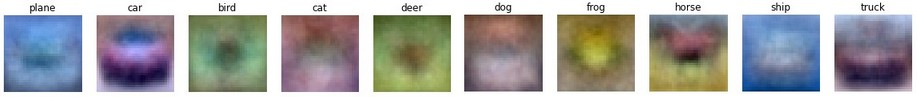
\includegraphics[width=\textwidth]{img/templates.jpg}
    \caption{Using gradient descent, the weights $\textbf{w}$ learn a visual resemblance of a class}
    \end{figure}
    \begin{itemize}
        \item Now, what do you think you this is a problem with these templates?
    \end{itemize}
     \footnotetext{cs231n.github.io/linear-classify}
\end{frame}

\begin{frame}{Image Classification}
    \begin{figure}
    \centering
    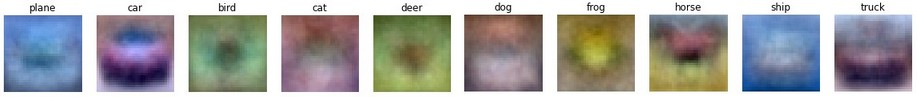
\includegraphics[width=\textwidth]{img/templates.jpg}
    \caption{Using gradient descent, the weights $\textbf{w}$ learn a visual resemblance of a class}
    \end{figure}
    \begin{itemize}
        \item Now, what do you think you this is a problem with these templates?
        \item It is very hard to capture all possible variations of an image using just a single template.
    \end{itemize}
     \footnotetext{cs231n.github.io/linear-classify}
\end{frame}

\section{Challenges of Computer Vision}
\begin{frame}{Challenges of Computer Vision}
\begin{itemize}
    \item Because images are very high-dimensional data, it is difficult for models to capture all possible variety and edge cases included in your data.
    \item Example: When using logistic regression, what happens when you shift an entire image left by one pixel?
\end{itemize}
\end{frame}

\begin{frame}{Challenges of Computer Vision}
\begin{figure}
    \centering
    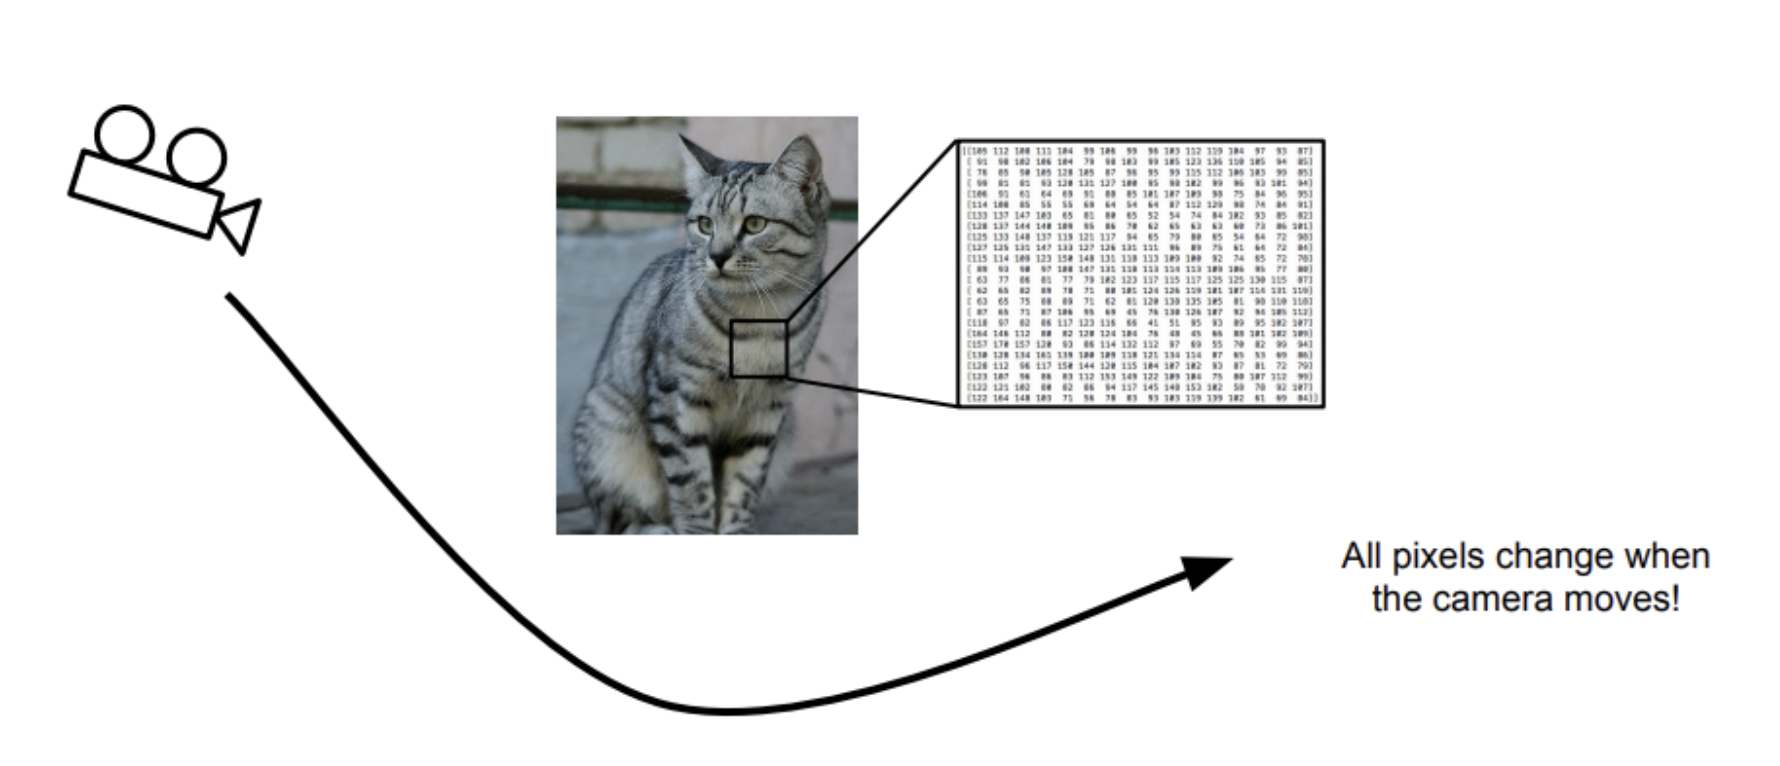
\includegraphics[width=0.9\textwidth]{img/viewpointvariation.png}
    \caption{Viewpoint Variation}
\end{figure}
\footnotetext{http://cs231n.stanford.edu/slides/2019/cs231n\_2019\_lecture02.pdf}
\end{frame}

\begin{frame}{Challenges of Computer Vision}
\begin{figure}
    \centering
    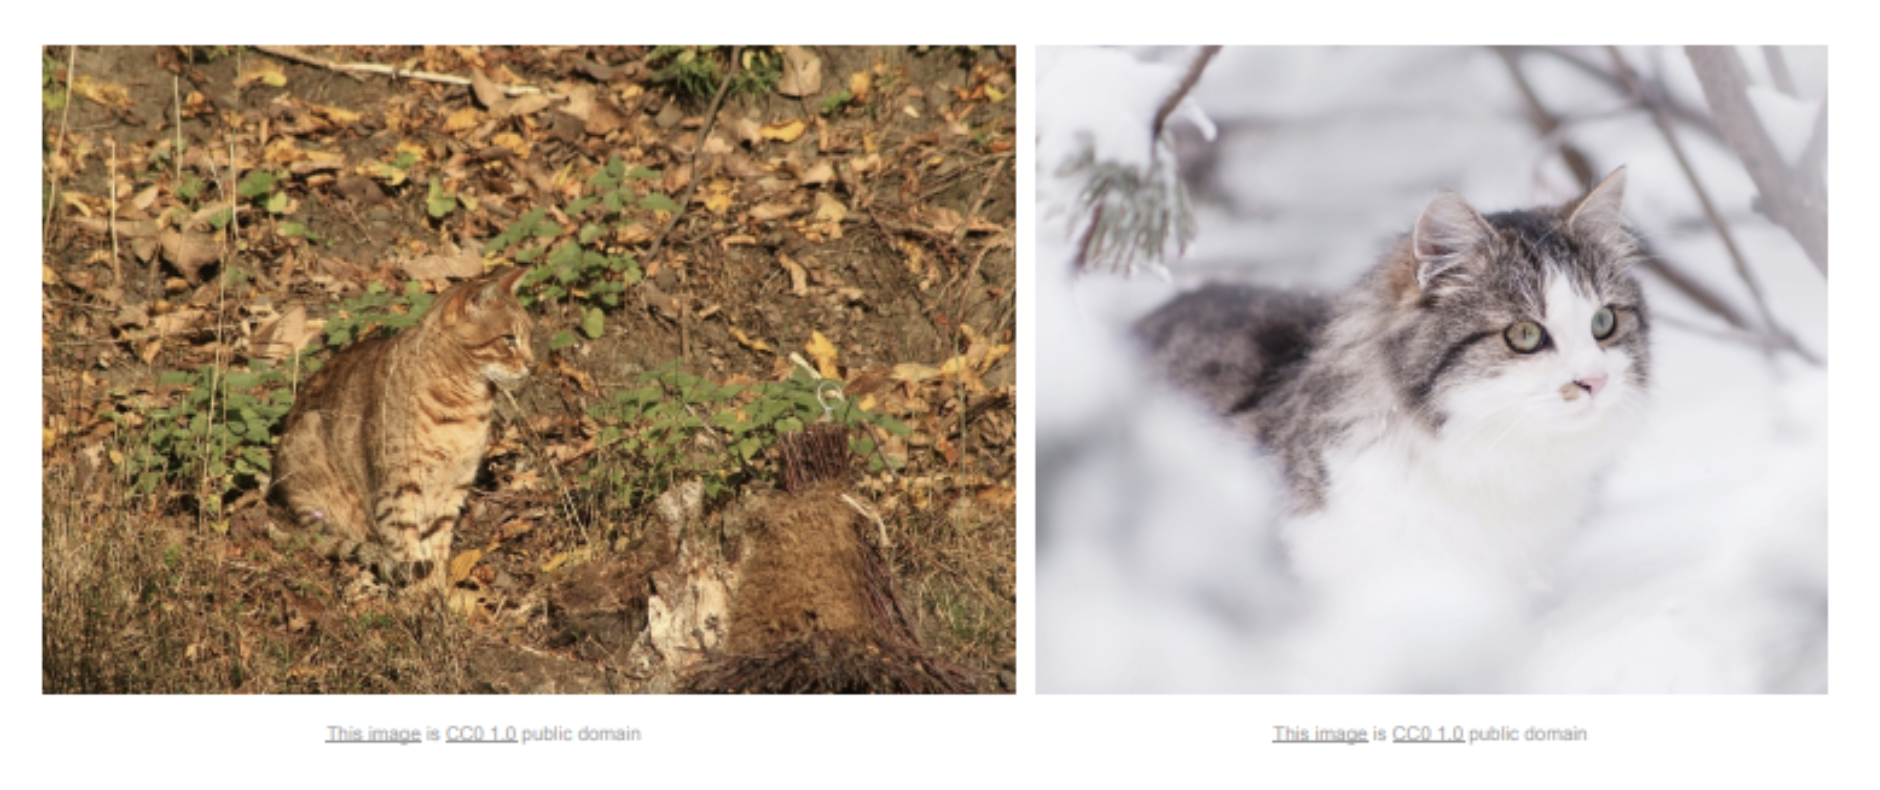
\includegraphics[width=0.9\textwidth]{img/occlusion.png}
    \caption{Background Clutter}
\end{figure}
\footnotetext{http://cs231n.stanford.edu/slides/2019/cs231n\_2019\_lecture02.pdf}
\end{frame}

\begin{frame}{Challenges of Computer Vision}
\begin{figure}
    \centering
    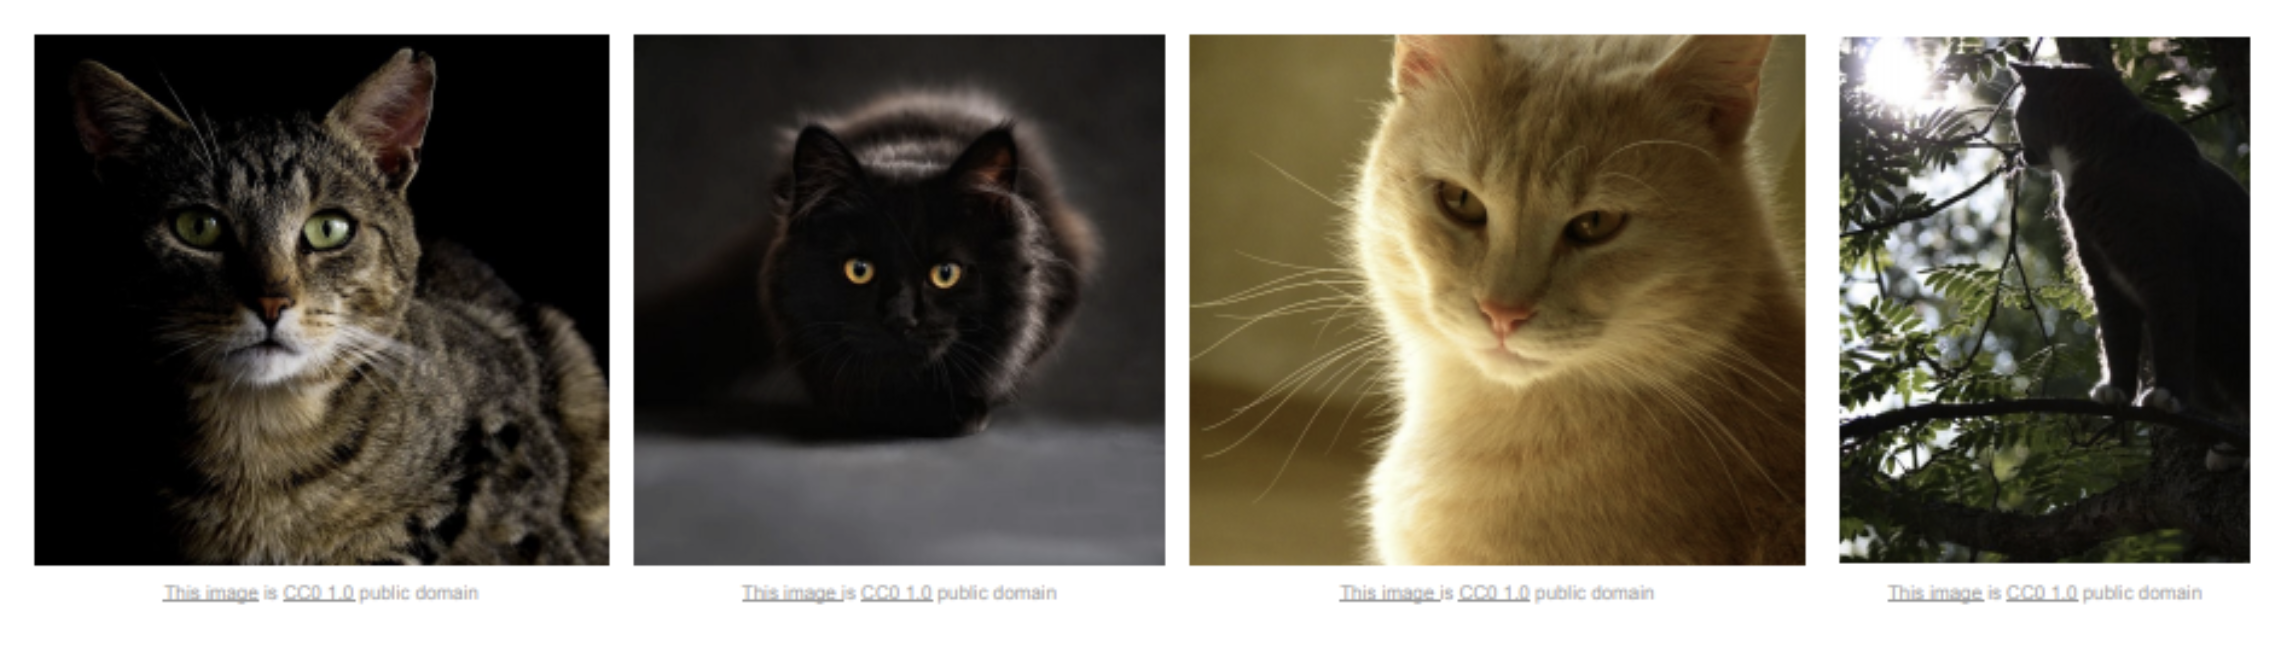
\includegraphics[width=0.9\textwidth]{img/illumination.png}
    \caption{Illumination}
\end{figure}
\footnotetext{http://cs231n.stanford.edu/slides/2019/cs231n\_2019\_lecture02.pdf}
\end{frame}

\begin{frame}{Challenges of Computer Vision}
\begin{figure}
    \centering
    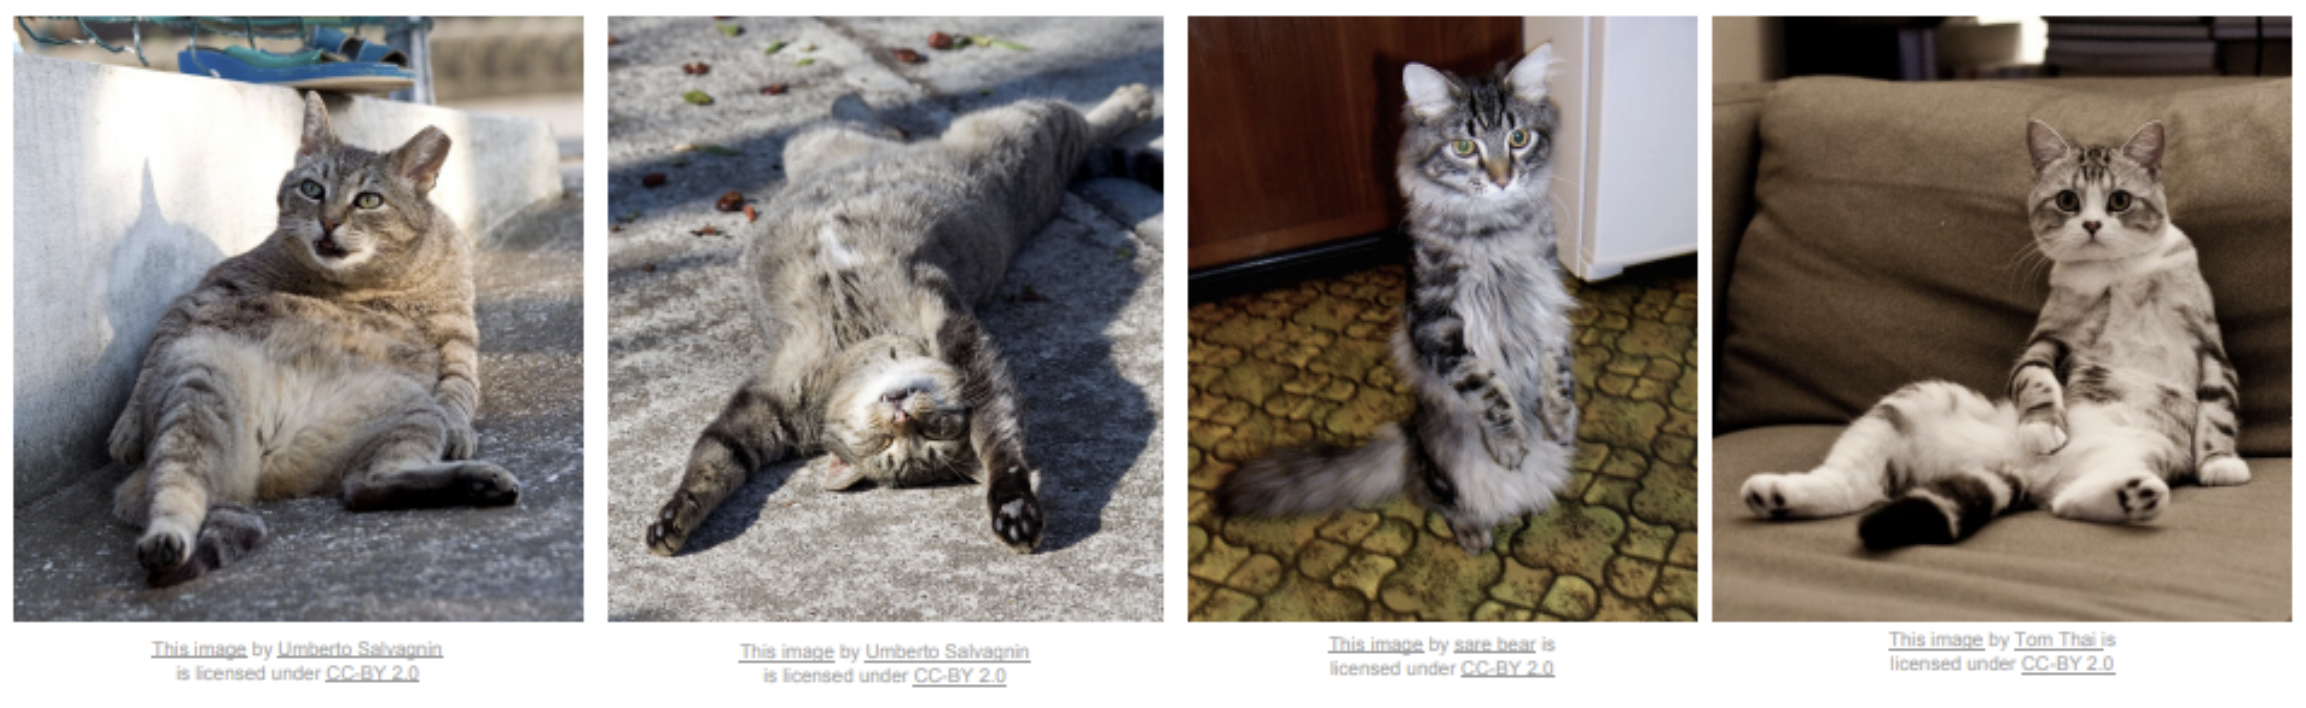
\includegraphics[width=0.9\textwidth]{img/deformation.png}
    \caption{Deformation}
\end{figure}
\footnotetext{http://cs231n.stanford.edu/slides/2019/cs231n\_2019\_lecture02.pdf}
\end{frame}

\begin{frame}{Challenges of Computer Vision}
\begin{figure}
    \centering
    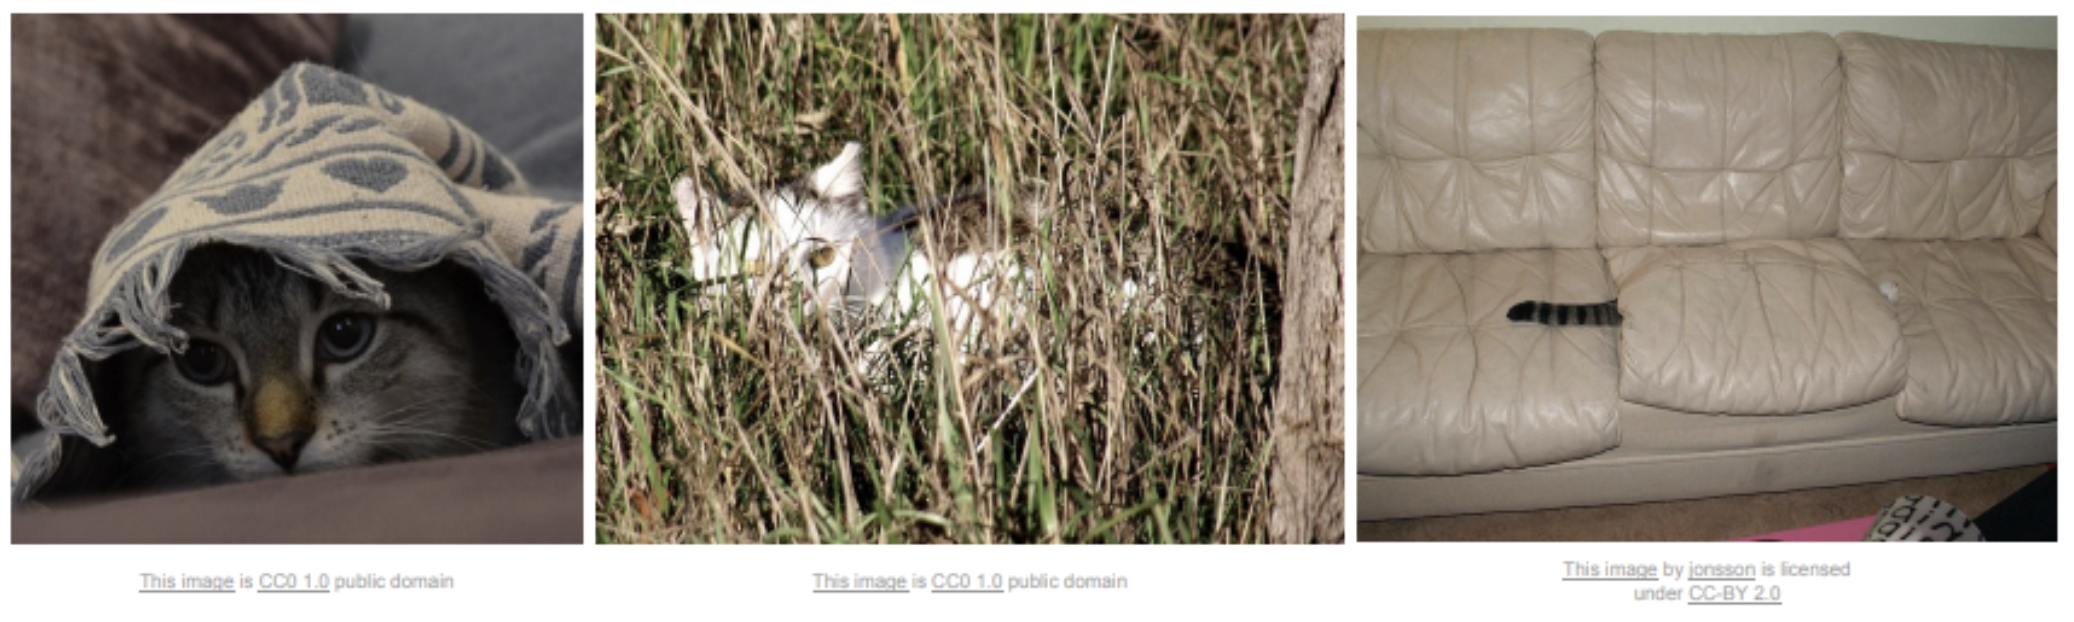
\includegraphics[width=0.9\textwidth]{img/hiding.png}
    \caption{Occlusion}
\end{figure}
\footnotetext{http://cs231n.stanford.edu/slides/2019/cs231n\_2019\_lecture02.pdf}
\end{frame}

\section{Neural Networks}
\begin{frame}{Neural Networks}
\begin{figure}
    \centering
    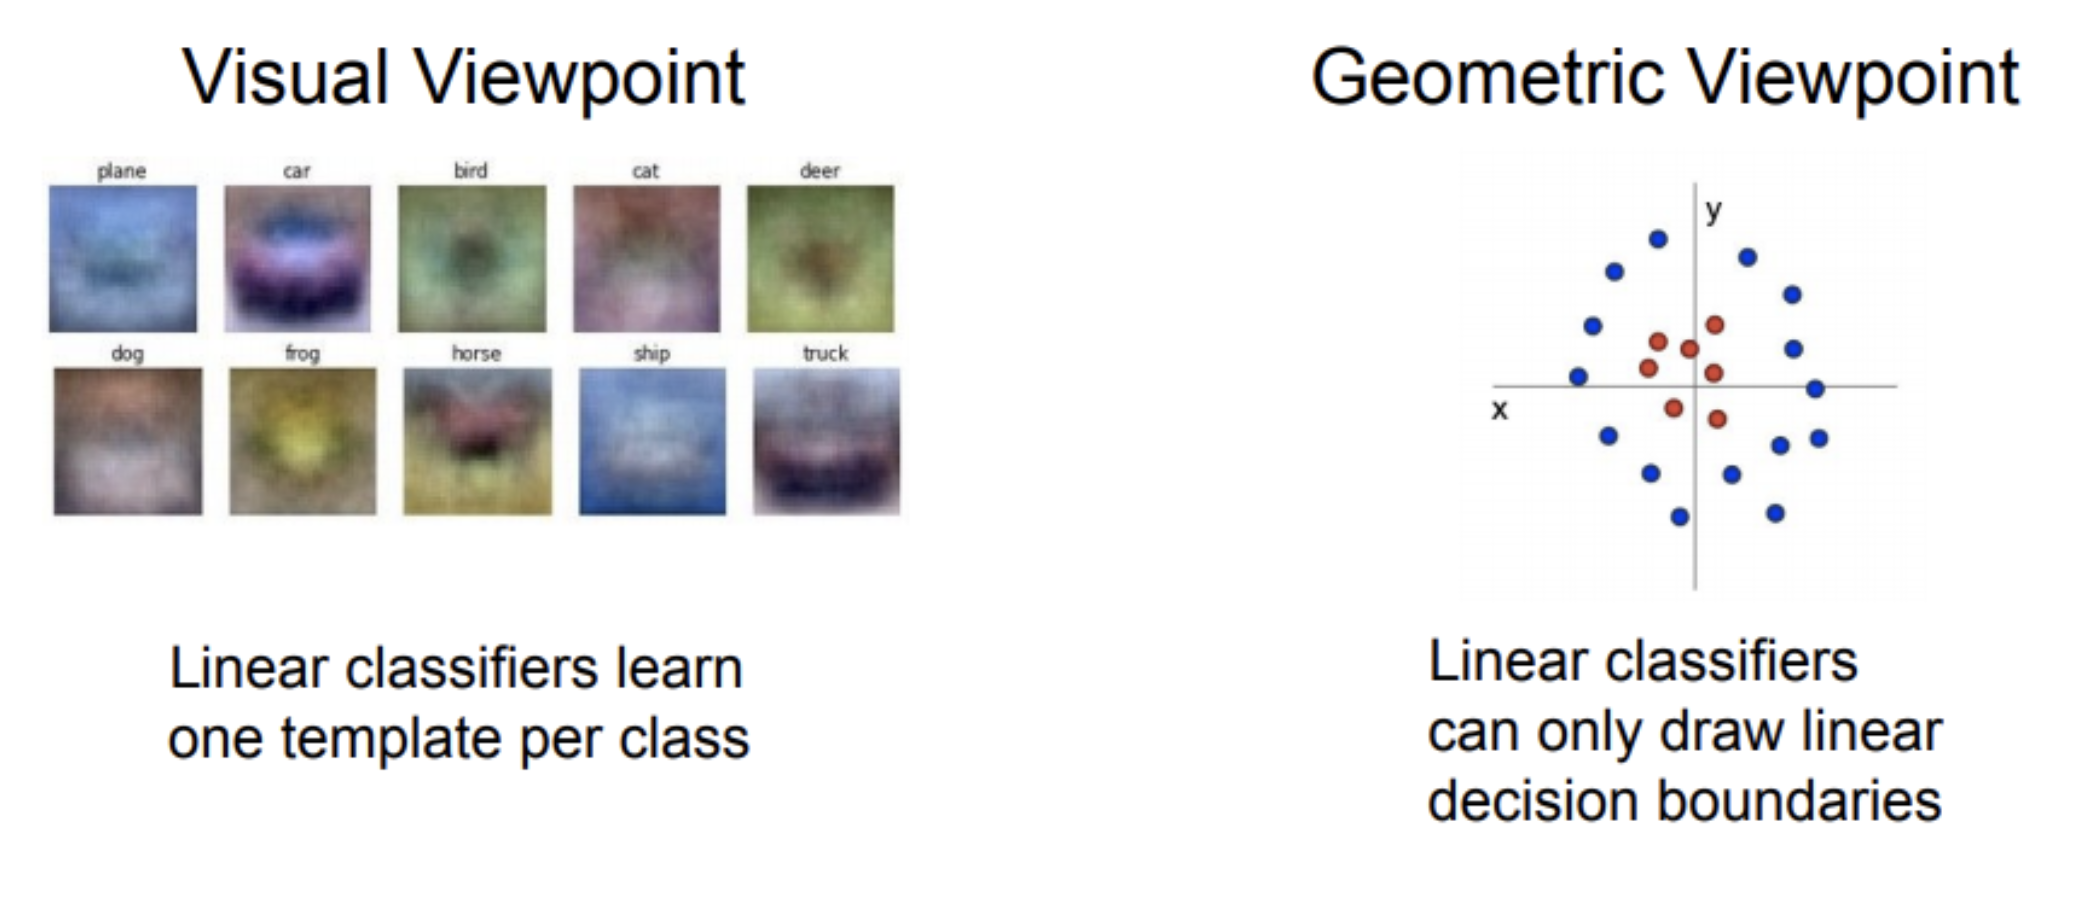
\includegraphics[width=\textwidth]{img/linearweak.png}
    \caption{Motivation: Linear models are fairly weak}
\end{figure}
\footnotetext{http://cs231n.stanford.edu/slides/2019/cs231n\_2019\_lecture02.pdf}
\end{frame}

\begin{frame}{Neural Networks}
\begin{itemize}
    \item We can model more complex functions by "stacking" more weights.
    \item Instead of
    $$\hat{y} = \sigma(\textbf{w} \cdot \textbf{x})$$
    We can now also do this:
    $$\hat{y} = \sigma(\textbf{w}_1 \cdot \sigma(\textbf{w}_2 \cdot \textbf{x}))$$
    $$\textbf{w}_1 \in \mathbf{R}^M, \textbf{w}_2 \in \textbf{R}^{M \times D}, \textbf{x} \in \textbf{R}^D$$
    Each row of the matrix $\textbf{w}_2$ is called a "neuron"
\end{itemize}
\end{frame}

\begin{frame}{Neural Networks}
\begin{figure}
    \centering
    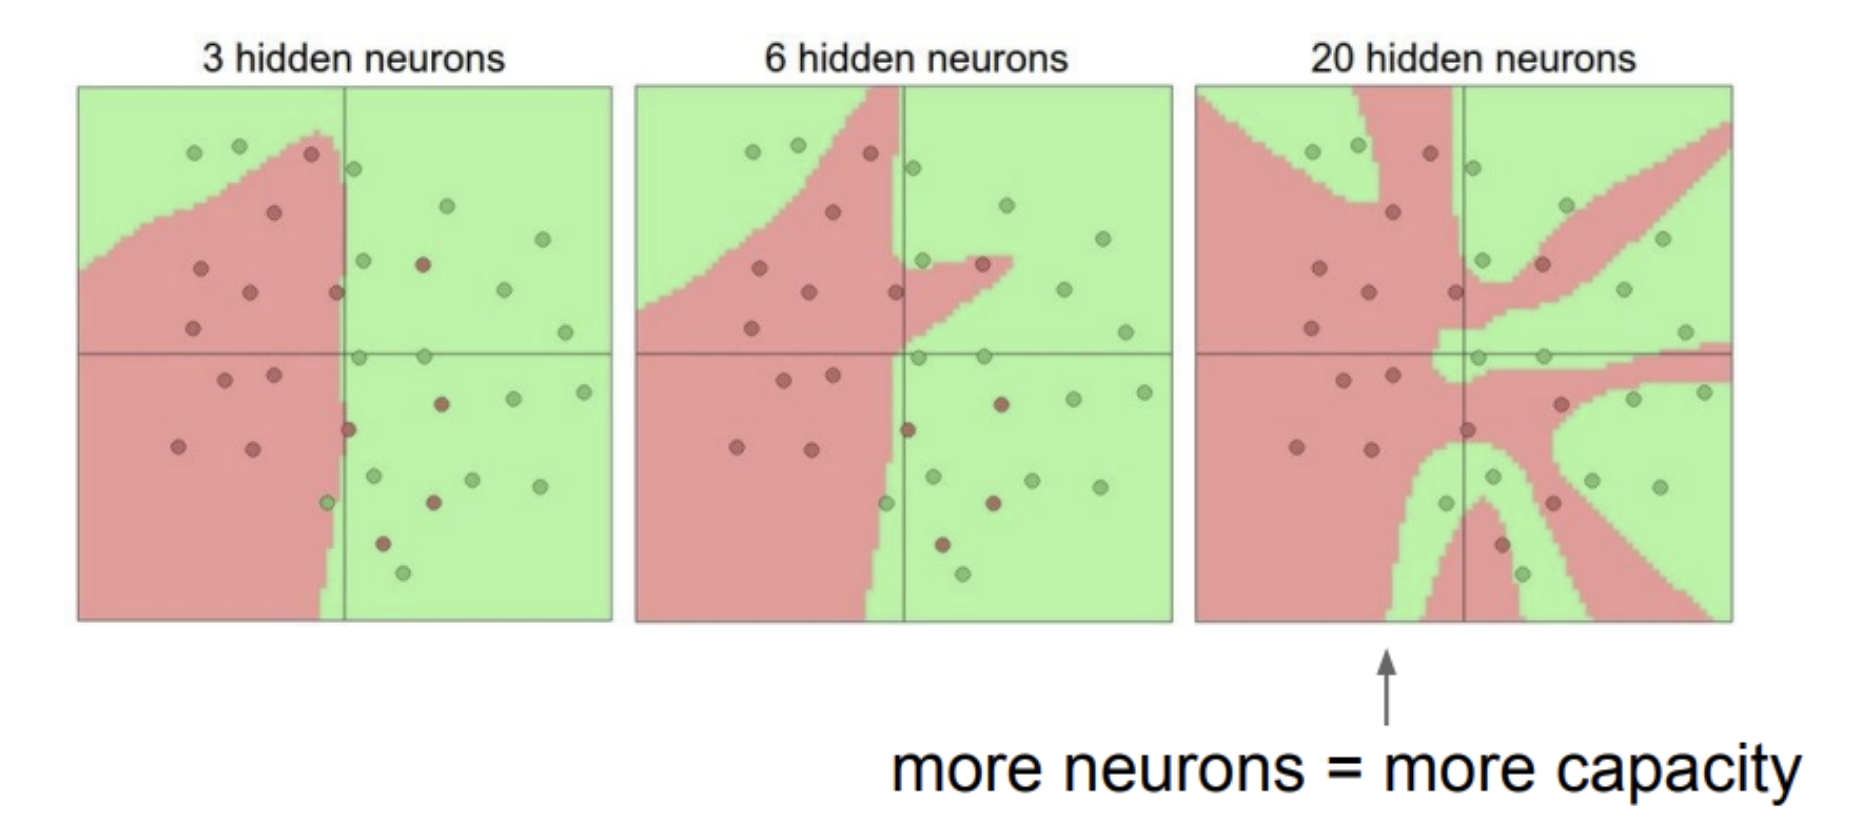
\includegraphics[width=0.8\textwidth]{img/moreneuronmorecap.png}
    \caption{The more neurons you have, the more \textbf{expressive} your model is.}
\end{figure}
\footnotetext{http://cs231n.github.io/neural-networks-1/}
\end{frame}

\begin{frame}{Neural Networks}
\begin{figure}
    \centering
    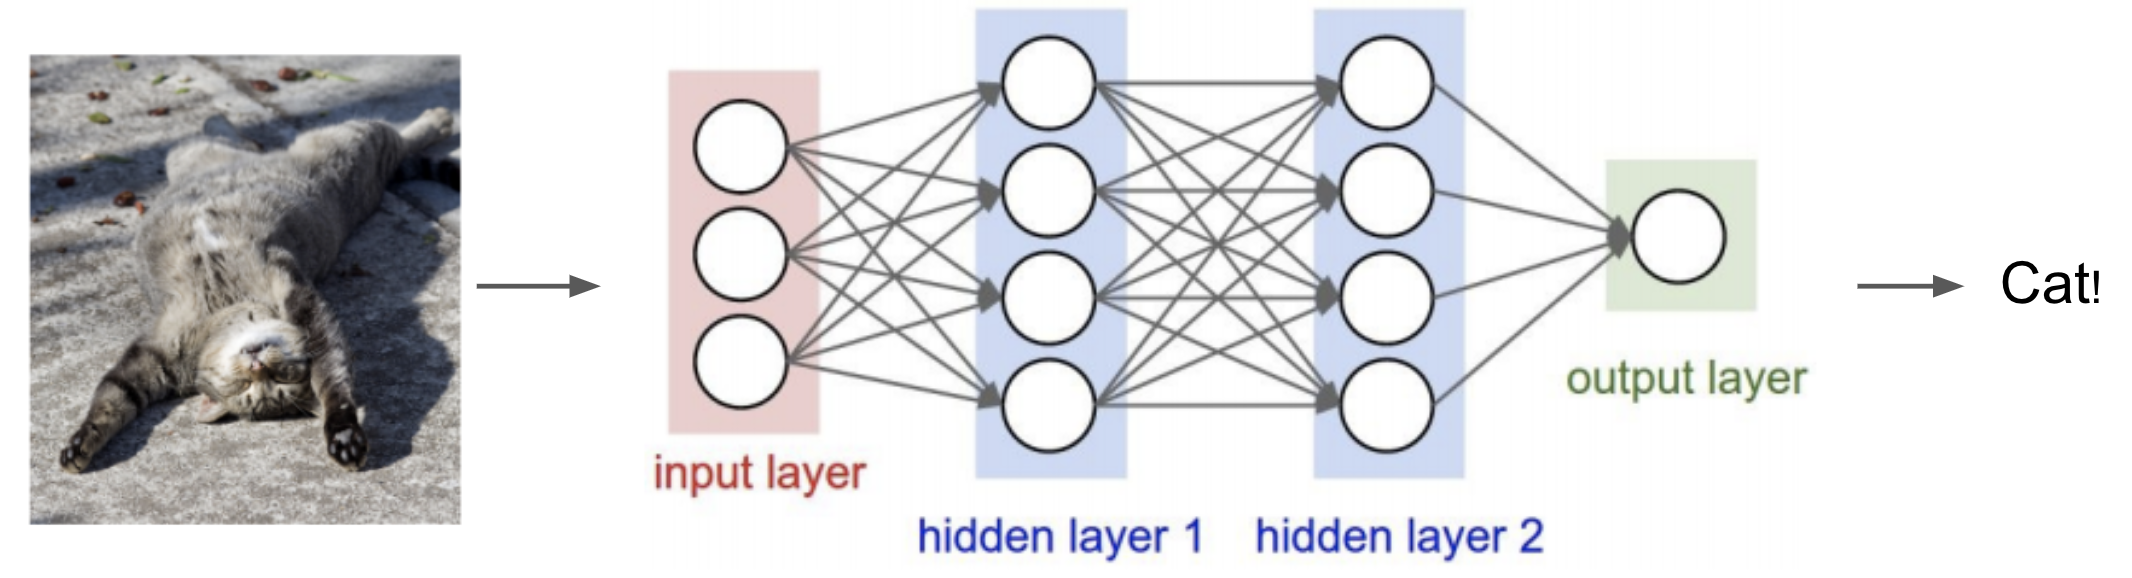
\includegraphics[width=\textwidth]{img/catNN.png}
    \caption{By stacking more and more layers and adding neurons, we can get models capable of representing all cats!}
\end{figure}
\end{frame}

%%%%%%%% repeat first slide %%%%%%%%
\begin{frame}
\titlepage 
\end{frame}
\end{document}